%Failed Attempts to Establish IPM for Asian Cycad Scale and Coconut Rhinoceros Beetle on Guam
%
%Aubrey Moore
%
%Guam's ecosystems are under attack by invasive species. Many people know about extinction of Guam's birds by the brown tree snake which invaded the island shortly after WWII. But the contemporary ecological disaster which is currently happening in Guam's forests is not well known.
%In 2002 a US Forest Service survey found the endemic cycad, Cycas micronesica, to be the most abundant tree in Guam's forests and coconut palm, Cocos nucifera, to be the second most abundant tree. Both species are now under severe attack by invasive insect species.
%
%About 90% of C. micronesica trees have been killed by Asian cycad scale, Aulacaspis yasumatsui, first detected in 2003.  The predatory beetle, Rhyzobius lophanthae, was introduced and it is protecting mature plants but no seedlings are surviving.
%
%Coconut rhinoceros beetle, Oryctes rhinoceros, was first detected in 2007 and an uncontrolled outbreak of this pest is currently killing coconut palms throughout the island.  Following a failed eradication attempt, Oryctes rhinoceros nudivirus (OrNV) and Metarhizium majus fungus were introduced as biocontrol agents. OrNV unexpectedly failed as a biocontrol agent for CRB on Guam. Previously, this pathogen produced excellent results when released on Pacific Islands infested with CRB. Subsequent laboratory bioassays and genetic analysis showed that the CRB which invaded Guam belong to an OrNV resistant biotype named CRB-G which is involved in all recent invasions of CRB in the Pacific. The fungus, M. majus rapidly established and spread to CRB breeding sites throughout the island, with infection rates measured between 10% and 38%.  But this level of suppression was not enough to prevent the current outbreak which was triggered by abundant breeding sites left in the wake of Typhoon Dolphin which passed over Guam in May 2015. 
%
%Attempts to overcome these IPM failures will be discussed.

%\documentclass[show notes]{beamer}
%\documentclass[handout]{beamer}
\documentclass[]{beamer}

\usepackage{pgfpages}
\usepackage[utf8]{inputenc}
\usepackage[T1]{fontenc}
\usepackage{mathabx}
\usepackage{mathpazo}
\usepackage{eulervm}
\usepackage{natbib}
\usepackage{adjustbox}
\usepackage{booktabs}

\usepackage{colortbl}

\hypersetup{colorlinks=true, urlcolor=blue, linkcolor=white, citecolor=blue}

\usepackage{caption}
\captionsetup[figure]{labelformat=empty}% redefines the caption setup of the figures environment in the beamer class.

\usetheme{Madrid}
\definecolor{uog}{rgb}{0,.5,0}
\usecolortheme[named=uog]{structure}

\mode<handout>{
    \pgfpagesuselayout{4 on 1}[letterpaper] 
    \setbeameroption{show notes}
}


% The following code uses \AtBeginSection to place a frame with the section title (\insertsectionhead) inside a beamercolorbox.
% From https://tex.stackexchange.com/questions/178800/creating-sections-each-with-title-pages-in-beamers-slides
\AtBeginSection[]{
  \begin{frame}
  \vfill
  \centering
  \begin{beamercolorbox}[sep=8pt,center,shadow=true,rounded=true]{title}
    \usebeamerfont{title}\insertsectionhead\par%
  \end{beamercolorbox}
  \vfill
  \end{frame}
}


\title[IPM Failures on Guam]{Failed Attempts to Establish IPM for Asian Cycad Scale and Coconut Rhinoceros Beetle on Guam}

\author{Aubrey Moore}

\institute[University of Guam]{College of Natural and Applied Sciences\\University of Guam}

\titlegraphic{
\includegraphics[width=2cm]{big_g2.pdf}}

\date[]{Entomological Society of America Annual Meeting, Vancouver\\November 13, 2018}

\begin{document}

%\maketitle

\begin{frame}
	\scriptsize{Symposium: \textit{Newly Established Exotic Pests: Transitioning from Emergency Response to IPM}}
	\titlepage
\end{frame}

\begin{frame}
	\scriptsize{Symposium: \textit{Newly Established Exotic Pests: Transitioning from Emergency Response to IPM}}
	\titlepage
\end{frame}


%\begin{frame}{Outline}
%    \tableofcontents
%\end{frame}

\section{Introduction}

\begin{frame}{Guam}
    \adjincludegraphics[height=1.05\textheight,center]{Guam.jpg}
\end{frame}

\begin{frame}{Brown treesnake}
	\adjincludegraphics[height=0.85\textheight,center]{bts.jpg}
	\tiny{Courtesy of USGS}
\end{frame}

\begin{frame}{Forest Birds before BTS}
	\begin{figure}
		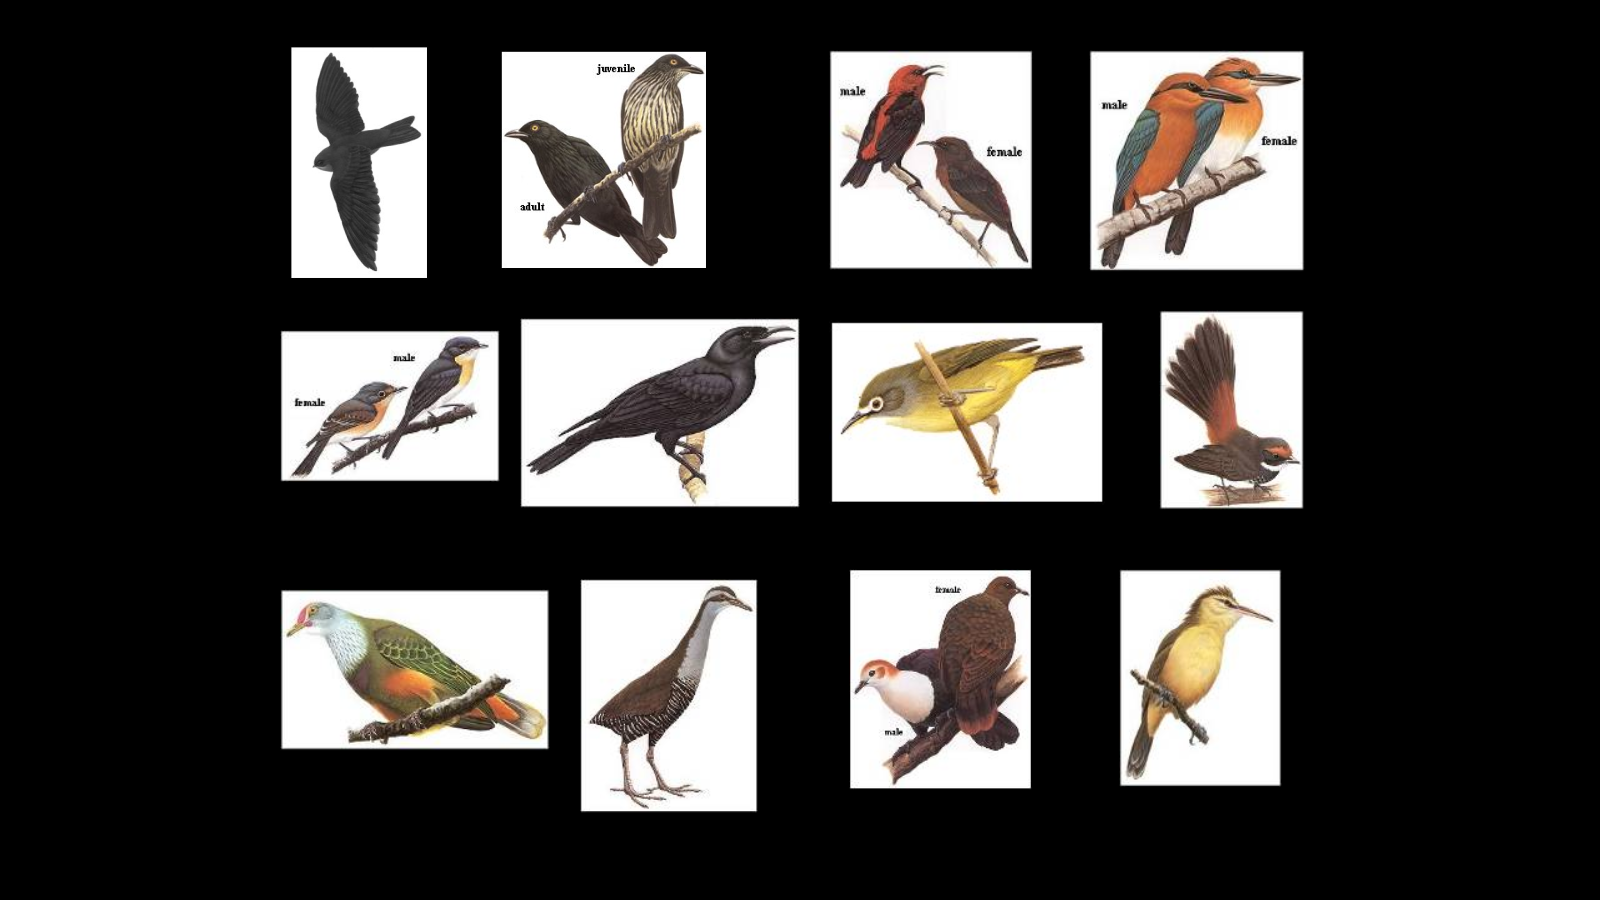
\includegraphics[height=0.8\textheight]{birds-before-bts.png}
	\end{figure}
\end{frame}

\begin{frame}{Forest Birds after BTS}
	\begin{figure}
		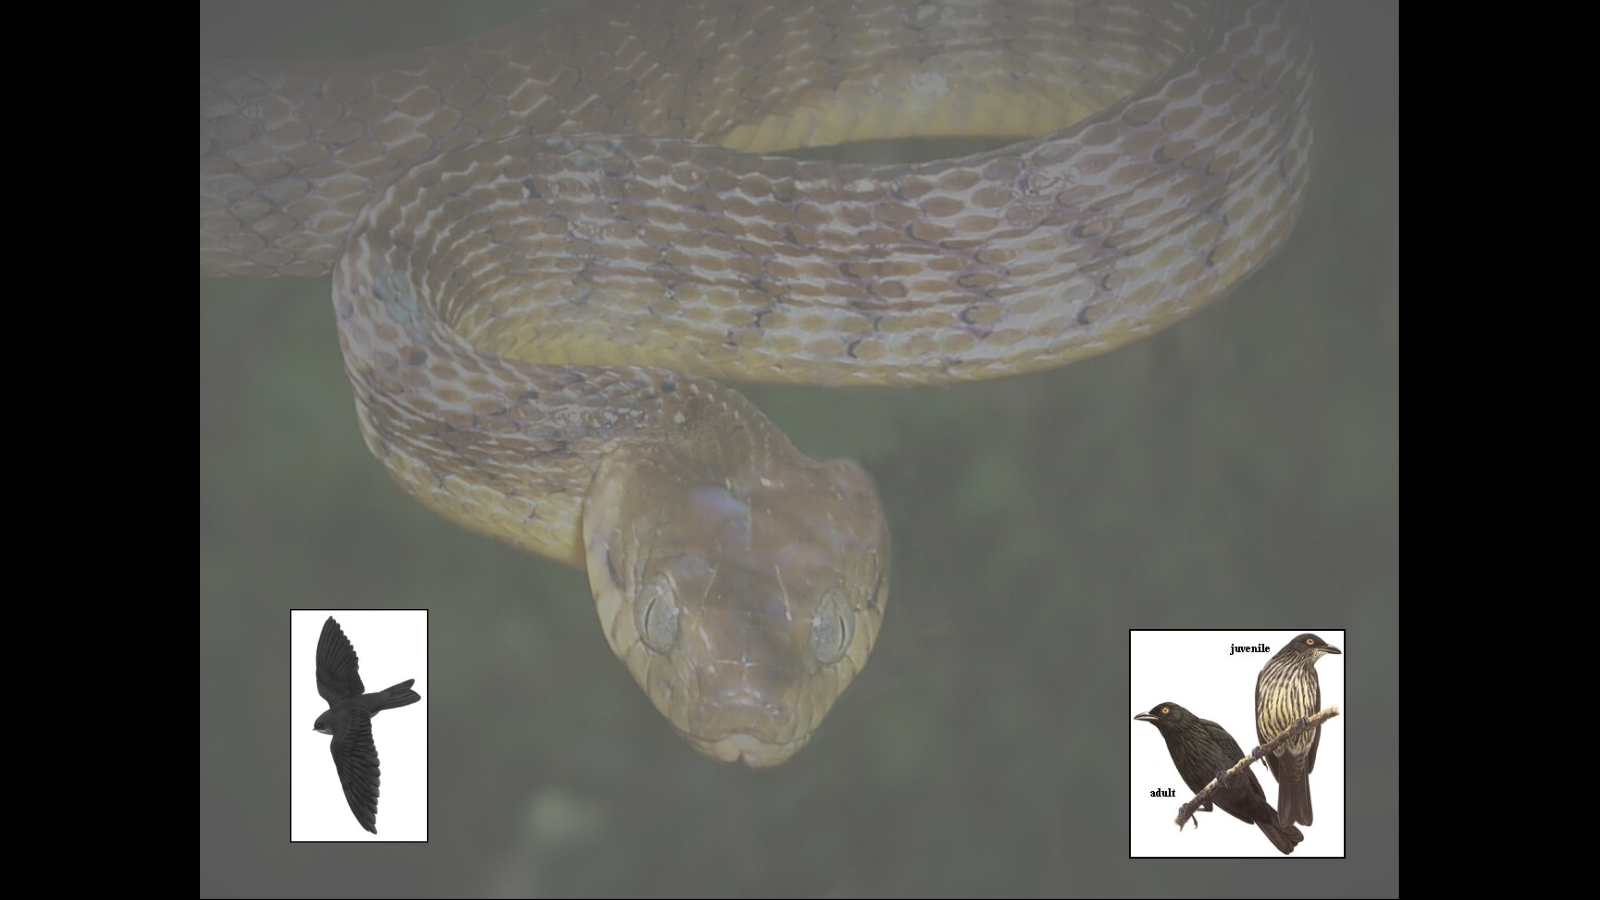
\includegraphics[height=0.8\textheight]{birds-after-bts.png}
	\end{figure}
\end{frame}

\begin{frame}{Loss of Ecosystem Services Provided by Birds}
	\begin{figure}
		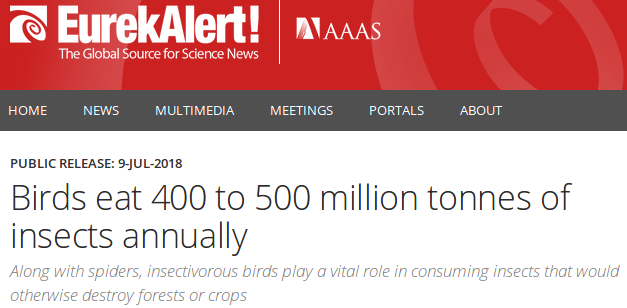
\includegraphics[height=0.5\textheight]{eureka-bird-loss.png}
	\end{figure}
	"Birds are an endangered class of animals ... we must fear that the vital ecosystem services that birds provide - such as the suppression of insect pests - will be lost." says Nyffeler.
	%\tiny{\url{https://link.springer.com/article/10.1007/s00114-018-1571-z#Sec10}}
\end{frame}


%\begin{frame}{HIPPO Threatens Guam's Biodiversity!}
%    \adjincludegraphics[height=\textheight,center]{hippo.jpg}
%\end{frame}
 
%\begin{frame}{HIPPO Threatens Guam's Biodiversity!}
%    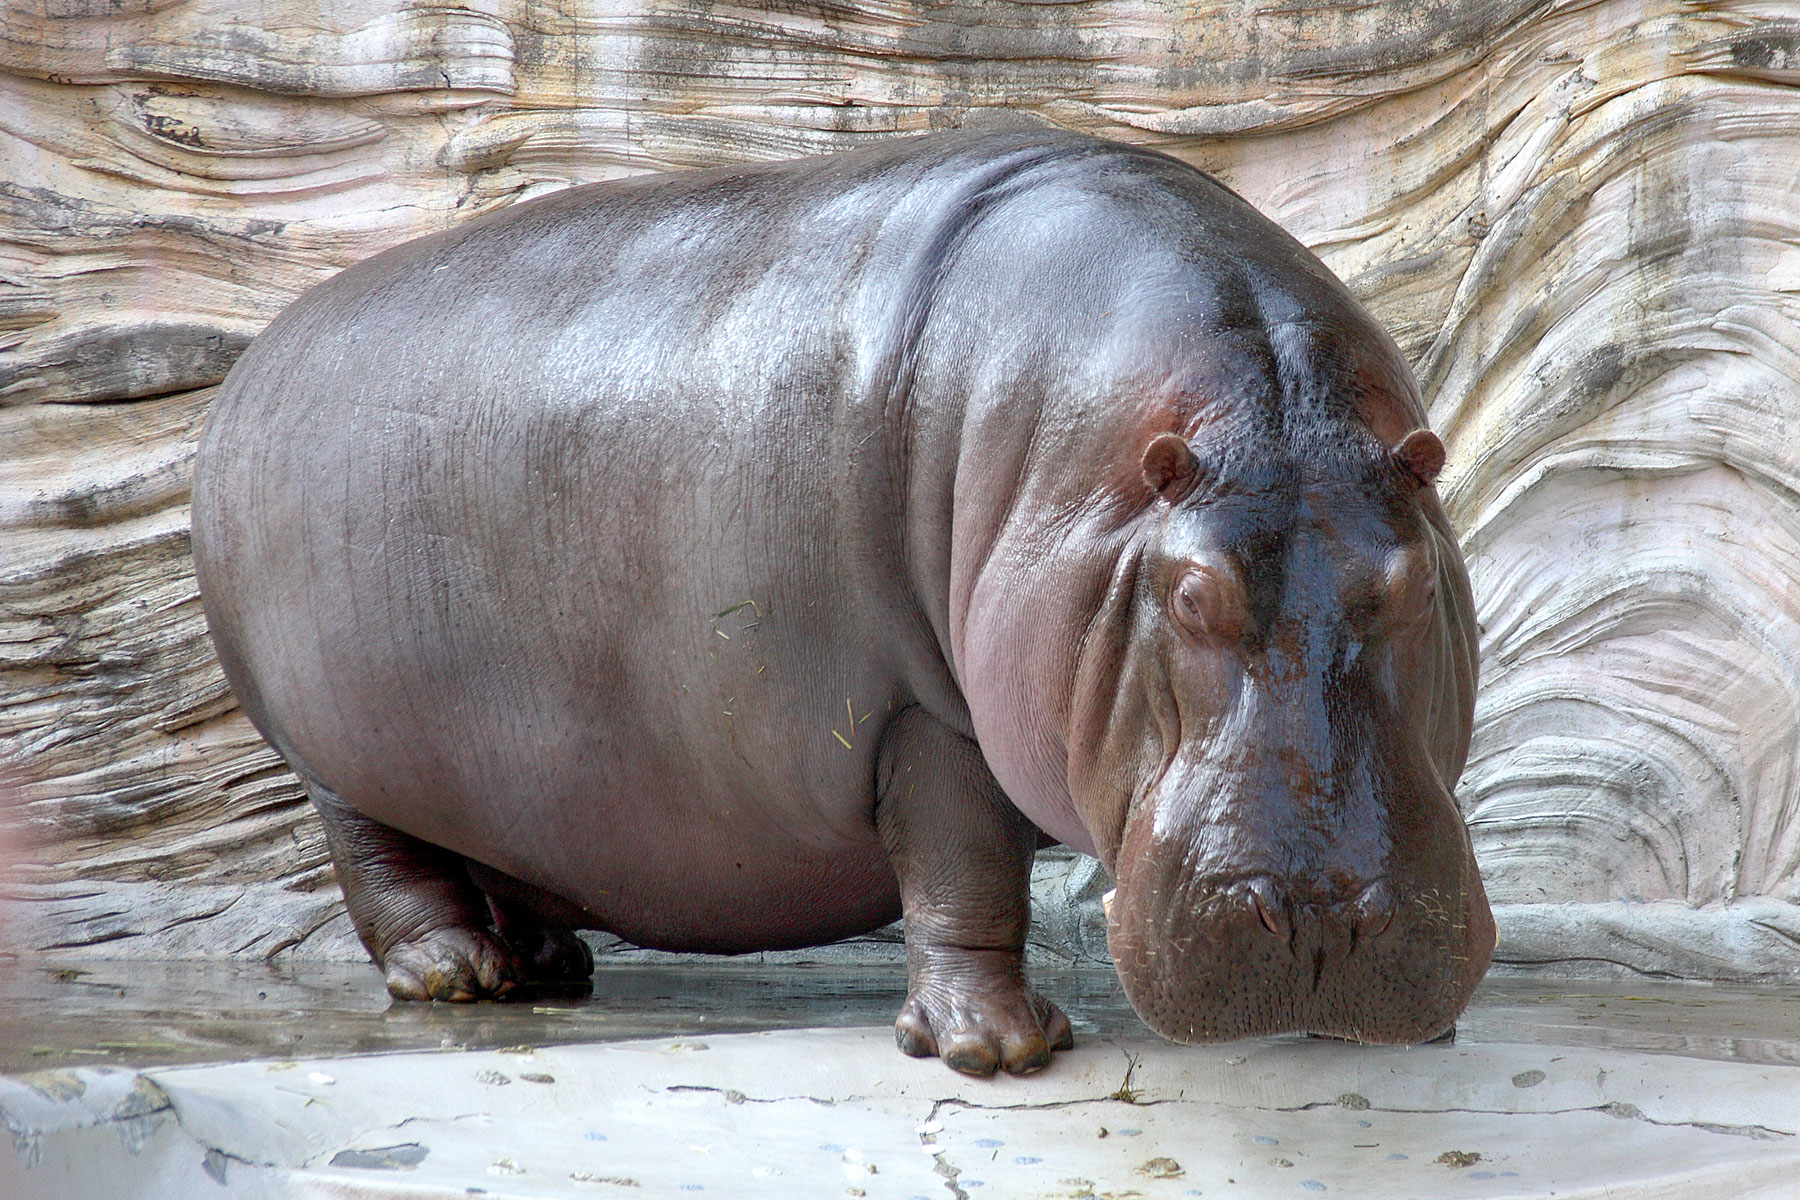
\includegraphics[height=0.5\textheight]{hippo.jpg}
%    \begin{description}
%        \item [\texttt{H}] Habitat loss
%        \item [\texttt{I}] Invasive Species
%        \item [\texttt{P}] Pollution 
%        \item [\texttt{P}] Human Population
%        \item [\texttt{O}] Overharvesting
%    \end{description}
%\end{frame}

\begin{frame}{Ecological Disasters on Guam}
	\begin{itemize}
		\item Brown treesnake (arrived around 1945)
		\begin{itemize}
			\item Killed most of Guam's birds and small mammals. 
			\item Caused 7 bird extinctions.
		\end{itemize}
		\item Asian Cycad Scale (detected 2003)
		\begin{itemize}
			\item Threatens survival of Guam's endemic cycad.
		\end{itemize}
		\item Coconut Rhinoceros Beetle (detected 2007). 
		\begin{itemize}
			\item Threatens Guam's coconuts and other palms.
		\end{itemize}
		\item Little Fire Ant (detected 2011)
		\begin{itemize}
			\item Threatens most animals remaining in Guam's forests.
		\end{itemize}
	\end{itemize}		
\end{frame}

\begin{frame}{Dominant Trees in Guam's Forests are Threatened by Asian Cycad Scale (ACS) and Coconut Rhinoceros Beetle (CRB)}
	\begin{center}
		\begin{tabular}{llcrp{0.35in}}
			\hline
			\textbf{Threat} & \textbf{Species} & \textbf{Status} & \textbf{Tree count\footnote{Estimated number of trees with DBH greater than 5 inches.}} & \textbf{\% of total tree count}\\
			\hline
			\rowcolor{yellow}
			ACS & \textit{Cycas micronesica} & endemic & 1,571,556 & 16\% \\ 
			\rowcolor{yellow}
			CRB & \textit{Cocos nucifera} & native & 1,162,494 & 12\% \\ 
			\rowcolor{yellow}
			CRB & \textit{Heterospathe elata} & introduced & 1,075,552 & 11\% \\ 
			
			\hline
			& \textit{Vitex parviflora} & introduced & 902,990 & 9\% \\ 
			& \textit{Leucaena leucocephala} & introduced & 890,217 & 9\%\\
			\hline
		\end{tabular} 
	\end{center}
	Tree census data source: J. A. Donnegon et al. 2004. Guam’s Forest Resources, 2002. Available from: \url{http://www.fs.fed.us/pnw/pubs/pnw_rb243.pdf}
	
\end{frame}

%\begin{frame}{Definition of 'Invasive Species'}
%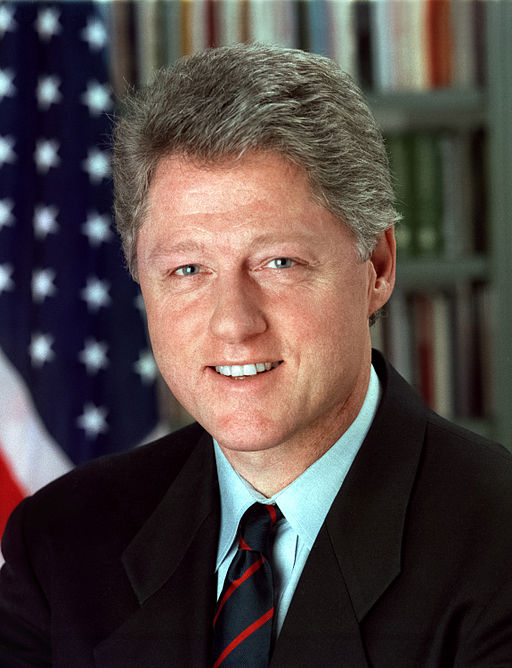
\includegraphics[height=0.4\textheight]{Bill_Clinton.jpg} \\
%
%\textbf{Invasive species} means an \textbf{alien}
%species whose introduction does or is
%likely to cause economic or
%environmental \textbf{harm} or harm to
%human health.
%
%\vspace{10px}
%Executive Order 13112
%
%President William Clinton
%
%February 3, 1999
%
%\vspace{10px}
%\textbf{invasive species} were previously referred to as \textbf{exotic pests}
%\end{frame}

%\begin{frame}{Small tropical islands are susceptable to damage by invasive species}
%\adjincludegraphics[height=0.6\textheight, center]{desert_island.jpg}
%\begin{itemize}
%\item no winter
%\item no predators, parasites, or diseases: 'escape from natural enemies'
%\end{itemize}
%\end{frame}

%\begin{frame}{Invasive Species Arrival Rate}
%	\begin{figure}
%		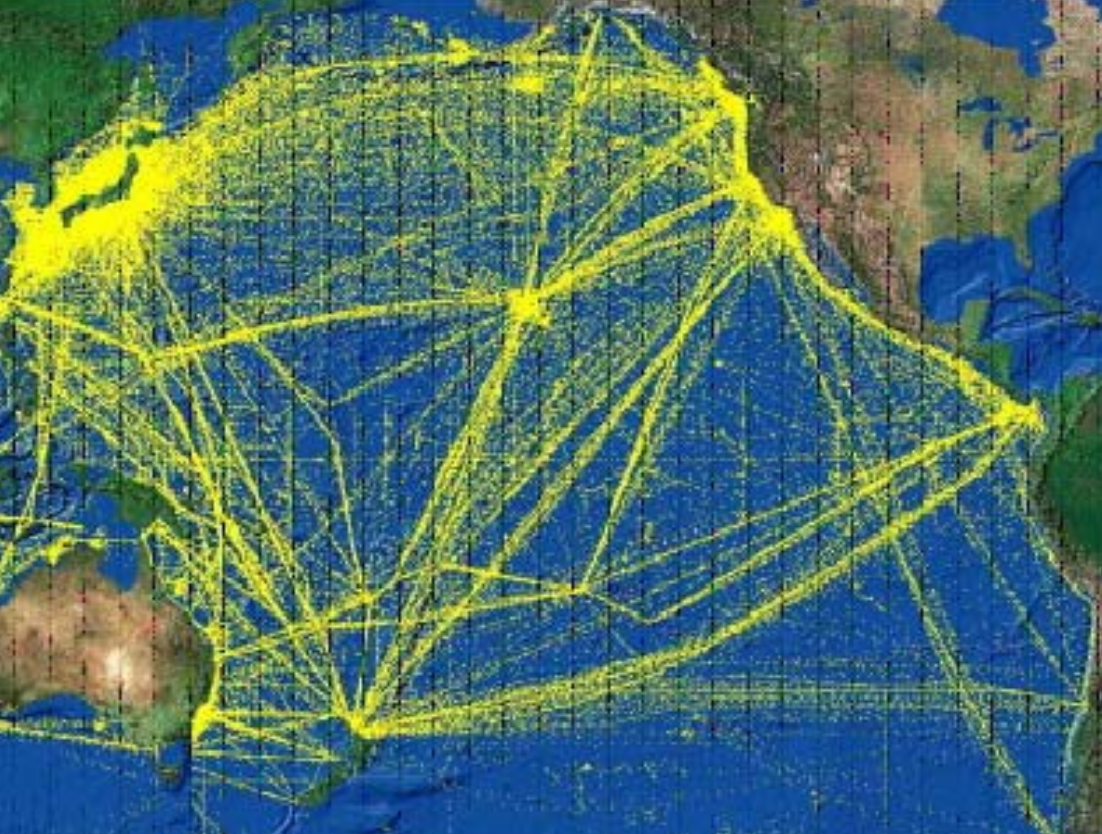
\includegraphics[width=0.5\textwidth]{pacific-traffic.png}
%		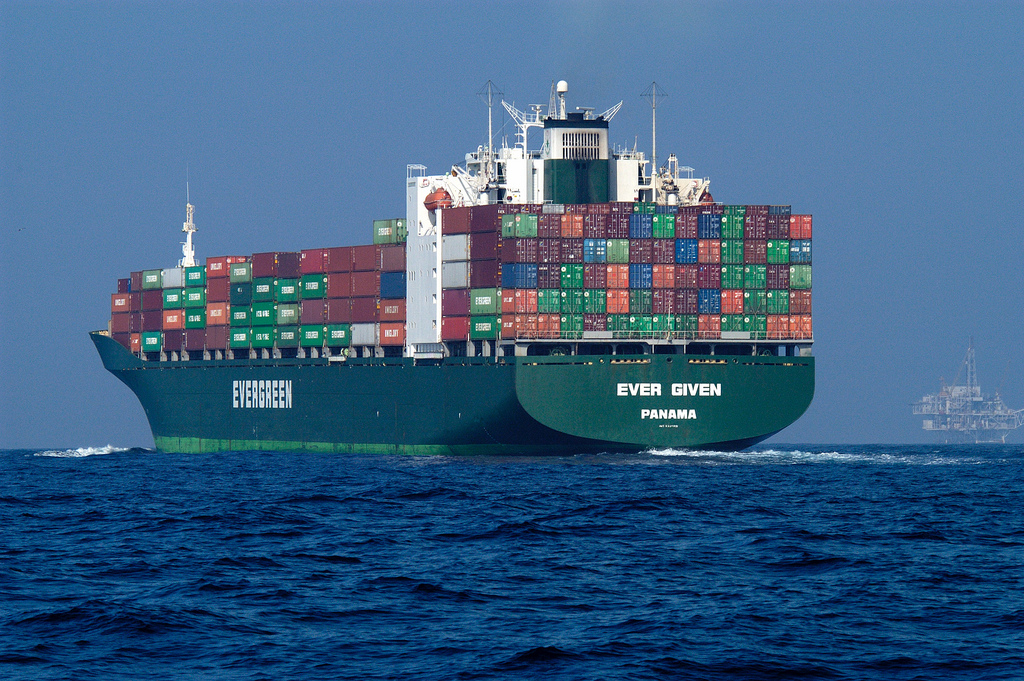
\includegraphics[width=0.5\textwidth]{container-ship.jpg}
%		\caption{Rate of invasive species arrivals is correlated with \textbf{globalization} and \textbf{containerization}.}
%	\end{figure}
%\end{frame}

%\begin{frame}{Kahalui Airport Pest Risk Assessment (KARA)}
%	\begin{itemize}
%		\item comprehensive inspection of all agricultural produces was performed on 130 days between September 2000 and July 2001
%		\item specimens were identified to species
%	\end{itemize}
%	\begin{figure}
%		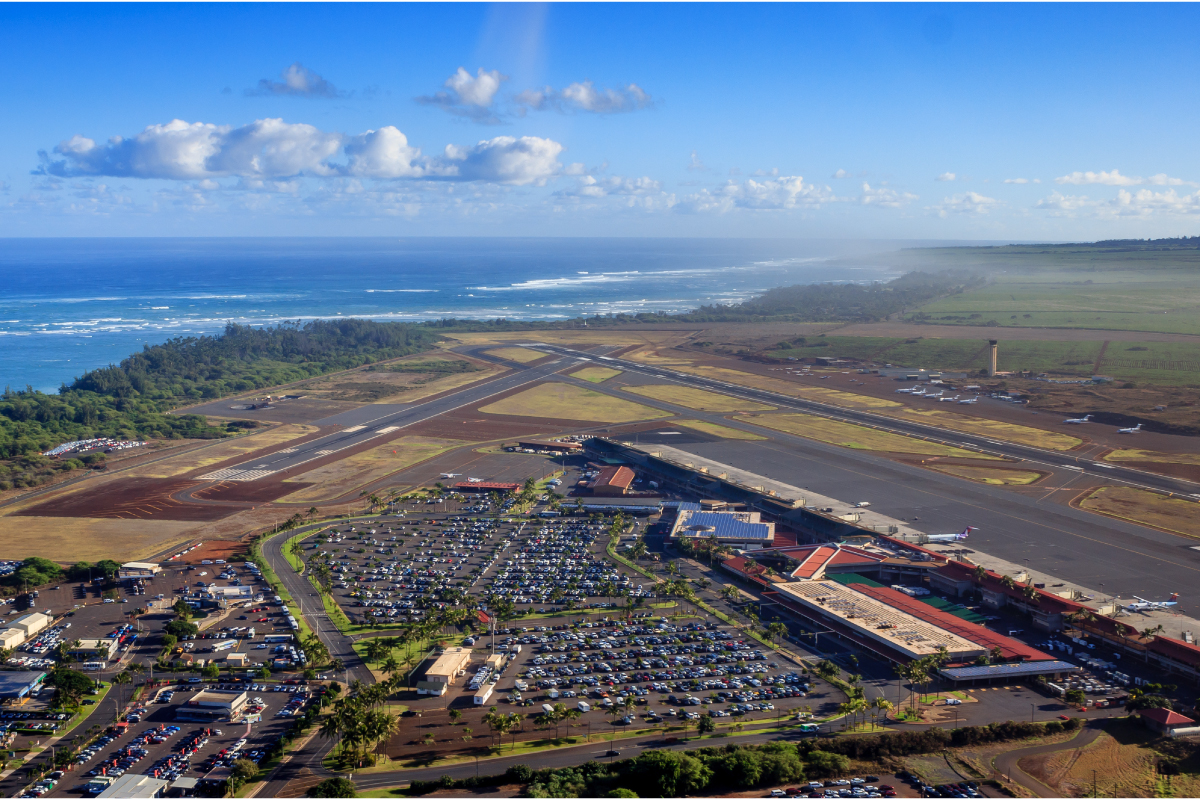
\includegraphics[height=0.35\textheight]{kahului-airport.jpg}
%	\end{figure}
%	\begin{itemize}
%		\item 125 species of pest insects and 16 plant diseases not known to occur in Hawaii were intercepted at Kahului during the 130 days of KARA inspections
%		\item \textbf{1 new invasive species arrived every day!}
%	\end{itemize}
%	\url{http://www.hawaiiag.org/PQ/KARA20Report20Final.pdf}
%\end{frame}

%\begin{frame}{Impact of invasive species on Guam}
%	\begin{itemize}
%		\item Almost all of Guam's pests are invasive species
%		\item One third of the "100 World's Worst Invasive Species" list published by the IUCN Invasive Species Specialist Group  occur on Guam
%	\end{itemize}
%\end{frame}

%\begin{frame}{Impediments to Dealing with Invasive Species on Guam}
%	\begin{itemize}
%		\item We suffer from the \textbf{Taxonomic Impediment}.
%		\item Professional capacity is inadequate.
%		\item Even when we manage to detect invasive species, our findings are rarely published in the scientific literature. 
%		\item Arrivals of and impacts of invasive species impacts on small islands are grossly under-reported.
%	\end{itemize}
%\end{frame}




%\section{Brown treesnake}




%\begin{frame}{BTS - Current Status}
%	\begin{itemize}
%		\item Millions of dollars per year are spent on preventing BTS from leaving Guam.
%		\item Some funds are being used for control methods development: snake-proof barriers and "pinkies on parachutes".
%	\end{itemize}
%\end{frame}

\section{Asian Cycad Scale}

\begin{frame}{Asian Cycad Scale (ACS), \textit{Aulacaspis yasumatsui}\\(Hemiptera: Diaspididae)}
	\begin{figure}
		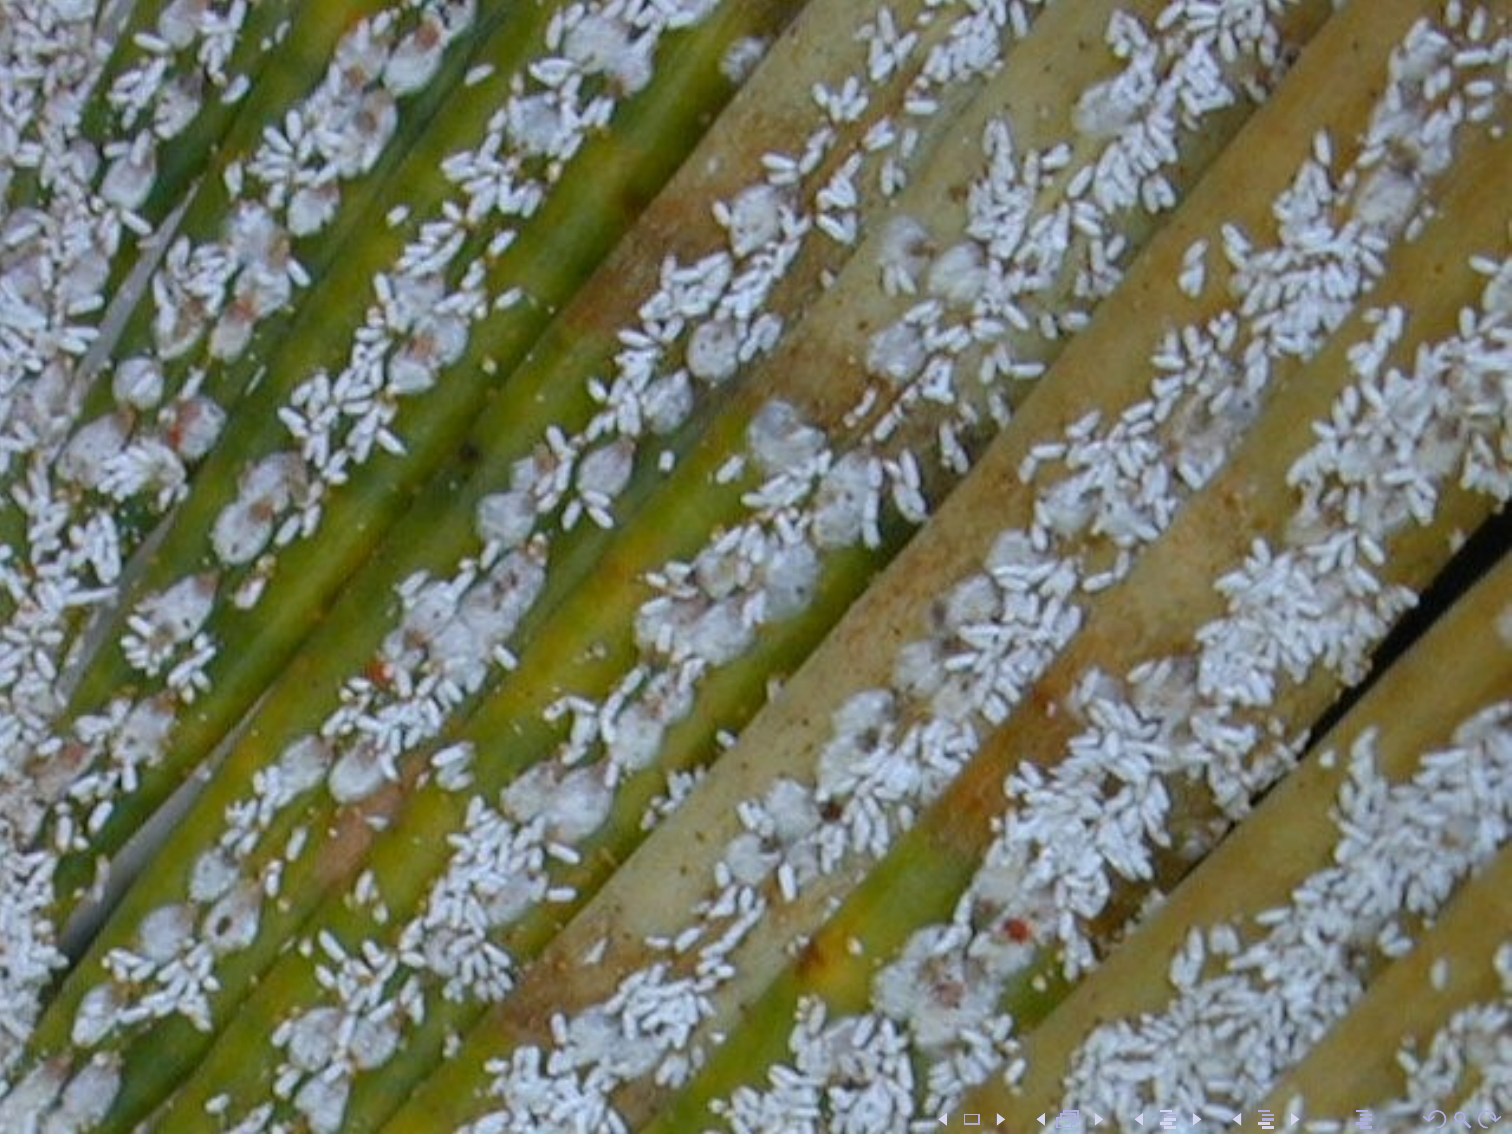
\includegraphics[height=0.7\textheight]{asian-cycad-scale/output-07.png}
	\end{figure}
\end{frame}


\begin{frame}{Biology}
\adjincludegraphics[width=\textwidth]{asian-cycad-scale/output-09.png}
\end{frame}

\begin{frame}{Invasion History}
	\begin{itemize}
		\item Origin: Southeast Asia
		\item Florida 1996
		\item Hawaii 1998
		\item Guam 2003
		\item Rota 2005
		\item Palau 2005
	\end{itemize}
\end{frame}

\begin{frame}{Damage to \textit{Cycas revoluta}}
	\adjincludegraphics[width=\textwidth]{asian-cycad-scale/output-14.png}
\end{frame}

\begin{frame}{Damage to \textit{Cycas micronesica}}
	\adjincludegraphics[width=\textwidth]{asian-cycad-scale/output-19.png}
\end{frame}

\begin{frame}{IPM Tactics for Asian Cycad Scale}
\begin{description}
	\item[Insecticides] can be used to protect ornamentals
	\item[Biocontrol] is the only feasable tactic for island-wide protection of \textit{Cycas micronesica}. A beetle predator has been introduced but attempts at introducing parasitoids have failed.
\end{description}
\end{frame}
%
%\begin{frame}{Current Efforts}
%	a
%\end{frame}

%\begin{frame}{09}
%	\adjincludegraphics[width=\textwidth]{asian-cycad-scale/output-09.png}
%\end{frame}

%\begin{frame}{10}
%	\adjincludegraphics[width=\textwidth]{asian-cycad-scale/output-10.png}
%\end{frame}
%
%\begin{frame}{11}
%	\adjincludegraphics[width=\textwidth]{asian-cycad-scale/output-11.png}
%\end{frame}
%
%\begin{frame}{12}
%	\adjincludegraphics[width=\textwidth]{asian-cycad-scale/output-12.png}
%\end{frame}
%
%\begin{frame}{13}
%	\adjincludegraphics[width=\textwidth]{asian-cycad-scale/output-13.png}
%\end{frame}
%
%\begin{frame}{14}
%	\adjincludegraphics[width=\textwidth]{asian-cycad-scale/output-14.png}
%\end{frame}
%
%\begin{frame}{15}
%	\adjincludegraphics[width=\textwidth]{asian-cycad-scale/output-15.png}
%\end{frame}
%
%\begin{frame}{16}
%	\adjincludegraphics[width=\textwidth]{asian-cycad-scale/output-16.png}
%\end{frame}
%
%\begin{frame}{17}
%	\adjincludegraphics[width=\textwidth]{asian-cycad-scale/output-17.png}
%\end{frame}
%
%\begin{frame}{18}
%	\adjincludegraphics[width=\textwidth]{asian-cycad-scale/output-18.png}
%\end{frame}
%
%\begin{frame}{19}
%	\adjincludegraphics[width=\textwidth]{asian-cycad-scale/output-19.png}
%\end{frame}
%
%\begin{frame}{20}
%	\adjincludegraphics[width=\textwidth]{asian-cycad-scale/output-20.png}
%\end{frame}
%

\begin{frame}{\textit{Rhyzobius lophanthae} (Coleoptera: Coccinellidae)}
	\adjincludegraphics[width=\textwidth]{asian-cycad-scale/output-25.png}
\end{frame}

\begin{frame}{\textit{Rhyzobius lophanthae} (Coleoptera: Coccinellidae)}
	\adjincludegraphics[width=\textwidth]{asian-cycad-scale/output-24.png}
\end{frame}

\begin{frame}{\textit{Arrhenophagus chionaspidus} (Hymnepotera: Encyrtidae)\\Fortuitous introduction 2013-02-10}
	\begin{center}	
	\adjincludegraphics[height=0.7\textheight]{arrhenophagus1.png}
	\adjincludegraphics[height=0.7\textheight]{arrhenophagus2.png}
	\end{center}
\end{frame}

%\begin{frame}{Massive mortality of \textit{Cycas micronesica} by invasive species}
%	\note[item]{Invasive species have killed about 90\% of Guam's endemic \textit{C. micronesica} plants and the population is not recovering}
%	\note[item]{\textit{C. micronesica} went from being the most numerous tree in Guam's forests in 2002 to being placed on the National Endangered Species list in 2016}
%	\adjincludegraphics[height=0.9\textheight,center]{CAS.png}
%\end{frame}

\begin{frame}{Asian Cycad Scale - Current Status on Guam}
	\begin{itemize}
		\item 90\% of Guam's endemic cycads have been killed by the scale and other invasive species
		
		\item \textit{Cycas micronesica} placed on the US National Endangered Species List in 2015. (Was the most abundant tree on Guam in 2002.)
				
		\item Mature plants are protected by the biocontrol beetle, but \textbf{no natural reproduction is occurring}
	\end{itemize}
\end{frame}


%\begin{frame}{Asian Cycad Scale - Origin and Pathway}
%	\begin{itemize}
%		\item Origin: Southeast Asia
%		\item Florida
%		\item Hawaii 1998
%		\item Guam 2003
%		\item Rota 2005?
%		\item Palau 2005?
%	\end{itemize}
%\end{frame}

%%%%


%%%%%

\section{Coconut Rhinoceros Beetle}

\begin{frame}{Coconut Rhinoceros Beetle Biotype-G (CRB)\\(Coleoptera: Scarabaeidae)}
\adjincludegraphics[width=\textwidth]{crbg.png}
\end{frame}

\begin{frame}{CRB Biotype G}
	\adjincludegraphics[width=\textwidth]{jip.png}
\end{frame}

\begin{frame}{CRB Biology}
	\adjincludegraphics[height=0.9\textheight,center]{crb_life_cycle2_cropped.png}
\end{frame}

\begin{frame}{CRB Damage 1}
	\adjincludegraphics[width=\textwidth]{crb-climate-change-connection/outputname-04.png}
\end{frame}

\begin{frame}{CRB Damage 2}
	\adjincludegraphics[width=\textwidth]{crb-climate-change-connection/outputname-05.png}
\end{frame}

\begin{frame}{CRB Breeding Sites}
	\adjincludegraphics[width=\textwidth]{crb-climate-change-connection/outputname-06.png}
\end{frame}

\begin{frame}{Coconut rhincoceros beetle}
	\adjincludegraphics[width=\textwidth]{crb-climate-change-connection/outputname-09.png}
\end{frame}

\begin{frame}{Coconut rhincoceros beetle}
	\adjincludegraphics[width=\textwidth]{crb-climate-change-connection/outputname-10.png}
\end{frame}


\begin{frame}{Invasion History: Coconut Rhinoceros Beetle Biotype G}
	\begin{itemize}
		\item Origin: Southeast Asia (Taiwan, Thailand, Philippines, Indonesia)
		\item Guam 2007
		\item Palau 2010
		\item Hawaii 2013
		\item Papua New Guinea 2015
		\item Solomon Islands 2015
		\item Rota 2017
	\end{itemize}
\end{frame}

\begin{frame}{IPM Tactics}
	\begin{description}
		\item[Eradication]Attempt based on sanitation and mass trapping failed when CRB-G spread throughout Guam
		\item[Sanitation]May be effective when practiced by a village community, but ineffective island-wide.
		\item[Pheromone traps]Ineffective for population suppression: mark-release-recapture indicates \textbf{oryctalure} traps have a capture rate of about 1\% of available adults
		\item[Insecticide application]\textbf{cypermethrin} can be used to protect palms
		\item[Biological control] is the only feasable tactic for island-wide control
				\begin{description}
					\item[\textit{Metarhizium majus} (GMF)]Successfully introduced from Philippines; survey indicates about 20\% from fungal infection
					\item[\textit{Oryctes rhinoceros} nudivirus (OrNV)]CRB-G is resistant to all available isolates
				\end{description}
				
	\end{description}
\end{frame}

%\begin{frame}{Coconut rhincoceros beetle}
%\adjincludegraphics[width=\textwidth]{crb-climate-change-connection/outputname-02.png}
%\end{frame}

%\begin{frame}{Geographic Distribution of Coconut Rhinoceros Beetle}
%\adjincludegraphics[width=\textwidth]{crb_map.png} \\
%\url{http://aubreymoore.github.io/crbdist/mymap.html}.
%\end{frame}
%
%\begin{frame}{Coconut Rhinoceros Beetle Life Cycle}
%	\adjincludegraphics[height=0.9\textheight,center]{crb_life_cycle2_cropped.png}
%\end{frame}
%
%
%\begin{frame}{Coconut rhincoceros beetle}
%\adjincludegraphics[width=\textwidth]{crb-climate-change-connection/outputname-08.png}
%\end{frame}

%%%


%%%

\begin{frame}{Coconut Rhinoceros Beetle - Current Status on Guam}
	\begin{itemize}
		\item Mature coconuts and other palms are rapidly being killed by an uncontrolled outbreak of CRB-G which was triggered by Typhoon Dolphin in 2016
		\item Damage estimates are not available. History suggests that we will loose 50\% or more of our palms if the outbreak is not controlled.
		\item A search for an effective biological control agent, most likely a new isolate of \textit{Oryctes rhinoceros} nudivirus is under way.
		\item If current outbreaks of CRB-G cannot be controlled, CRB-G will spread to other islands and possibly the Americas.
	\end{itemize}
\end{frame}

%\begin{frame}{LFA - Prognosis for Guam}
%	\begin{itemize}
%		\item A search for an effective biological control agent, most likely a new isolate of \textit{Oryctes rhinoceros} nudivirus is under way.
%	\end{itemize}
%\end{frame}

%\begin{frame}{Coconut rhincoceros beetle}
%\adjincludegraphics[width=\textwidth]{crb-climate-change-connection/outputname-14.png}
%\end{frame}
%
%\begin{frame}{Coconut rhincoceros beetle}
%\adjincludegraphics[width=\textwidth]{crb-climate-change-connection/outputname-13.png}
%\end{frame}
%
%\begin{frame}{Coconut rhincoceros beetle}
%\adjincludegraphics[width=\textwidth]{crb-climate-change-connection/outputname-15.png}
%\end{frame}

%\section{Little Fire Ant}
%
%\begin{frame}{LFA - Biology}
%	\begin{figure}
%	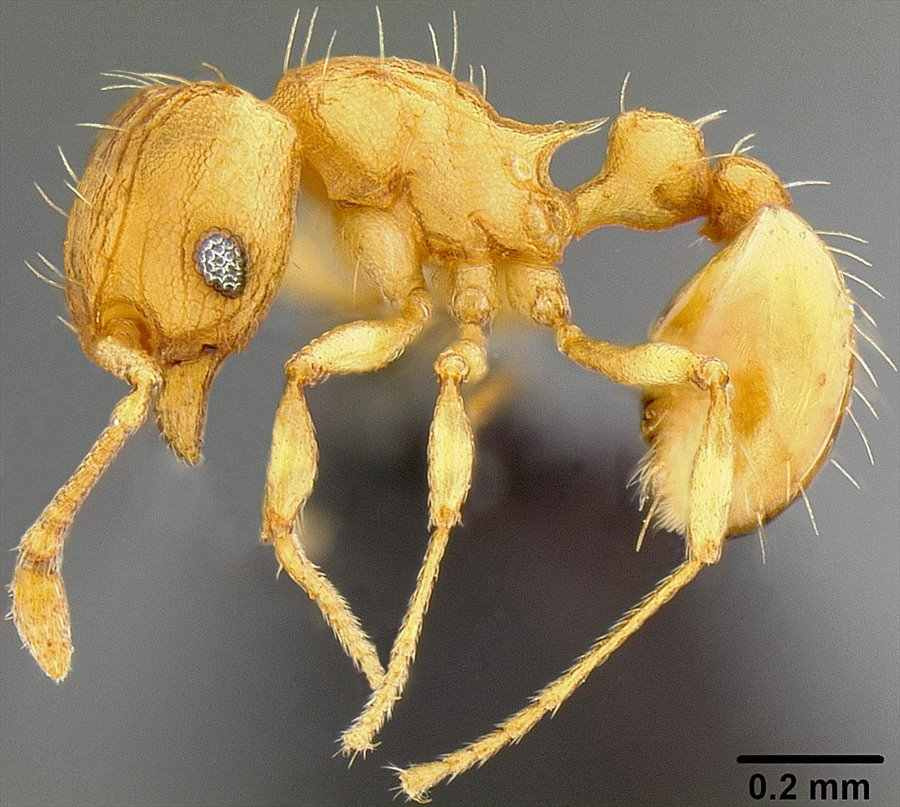
\includegraphics[height=0.6\textheight]{lfa.jpg}
%	\caption{Little fire ant, \textit{Wasmannia auropunctata} (HYMENOPTERA: FORMICIDAE)}
%	\end{figure}
%	\begin{itemize}
%		\item Forms supercolonies with multiple queens
%		\item Nests in trees and on ground
%	\end{itemize}
%\end{frame}
%
%\begin{frame}{LFA - Biology}
%\begin{figure}
%	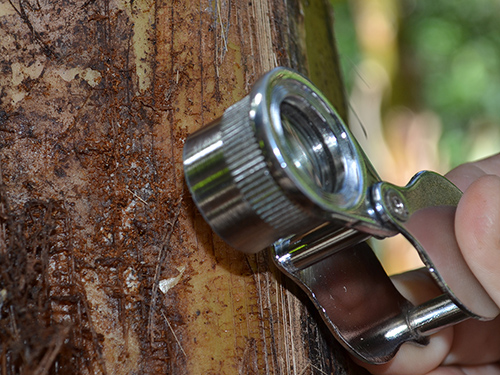
\includegraphics[width=0.5\textwidth]{lfa2small.jpg}
%	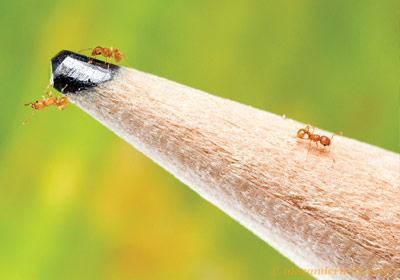
\includegraphics[width=0.5\textwidth]{lfa-pencil.jpg}
%	\caption{Little fire ants are little :)}
%\end{figure}
%\end{frame}
%
%\begin{frame}{LFA - Biology}
%\begin{figure}
%	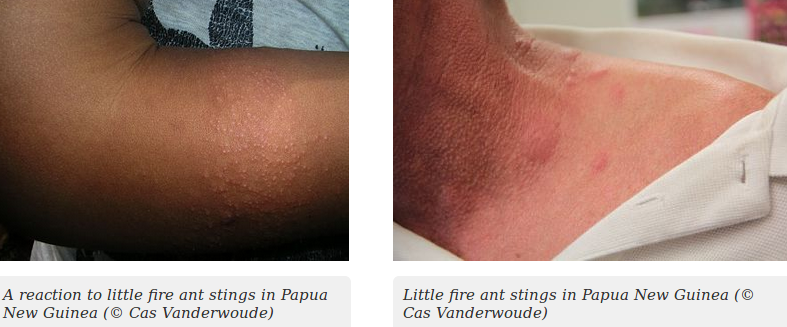
\includegraphics[width=\textwidth]{lfa-stings.png}
%\end{figure}
%\end{frame}
%
%\begin{frame}{LFA - Biology}
%\begin{figure}
%	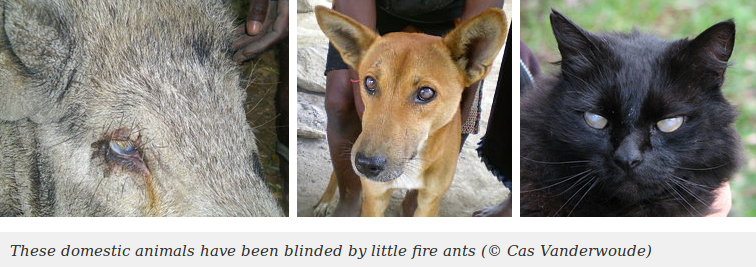
\includegraphics[width=\textwidth]{lfa-eyes.png}
%\end{figure}
%\end{frame}
%
%\begin{frame}{LFA - Biology}
%\begin{figure}
%	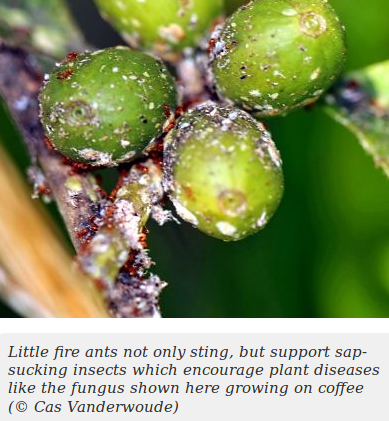
\includegraphics[height=0.85\textheight]{lfa-hemiptera.png}
%\end{figure}
%\end{frame}
%
%\begin{frame}{Little Fire Ant - Origin and Pathway}
%	\begin{itemize}
%		\item Origin: South America
%		\item Florida 1920s
%		\item Hawaii 1999
%		\item Guam 2011
%		\item Yap 2017
%	\end{itemize}
%\end{frame}
%
%\begin{frame}{LFA - Detection on Guam}
%	\begin{figure}	
%		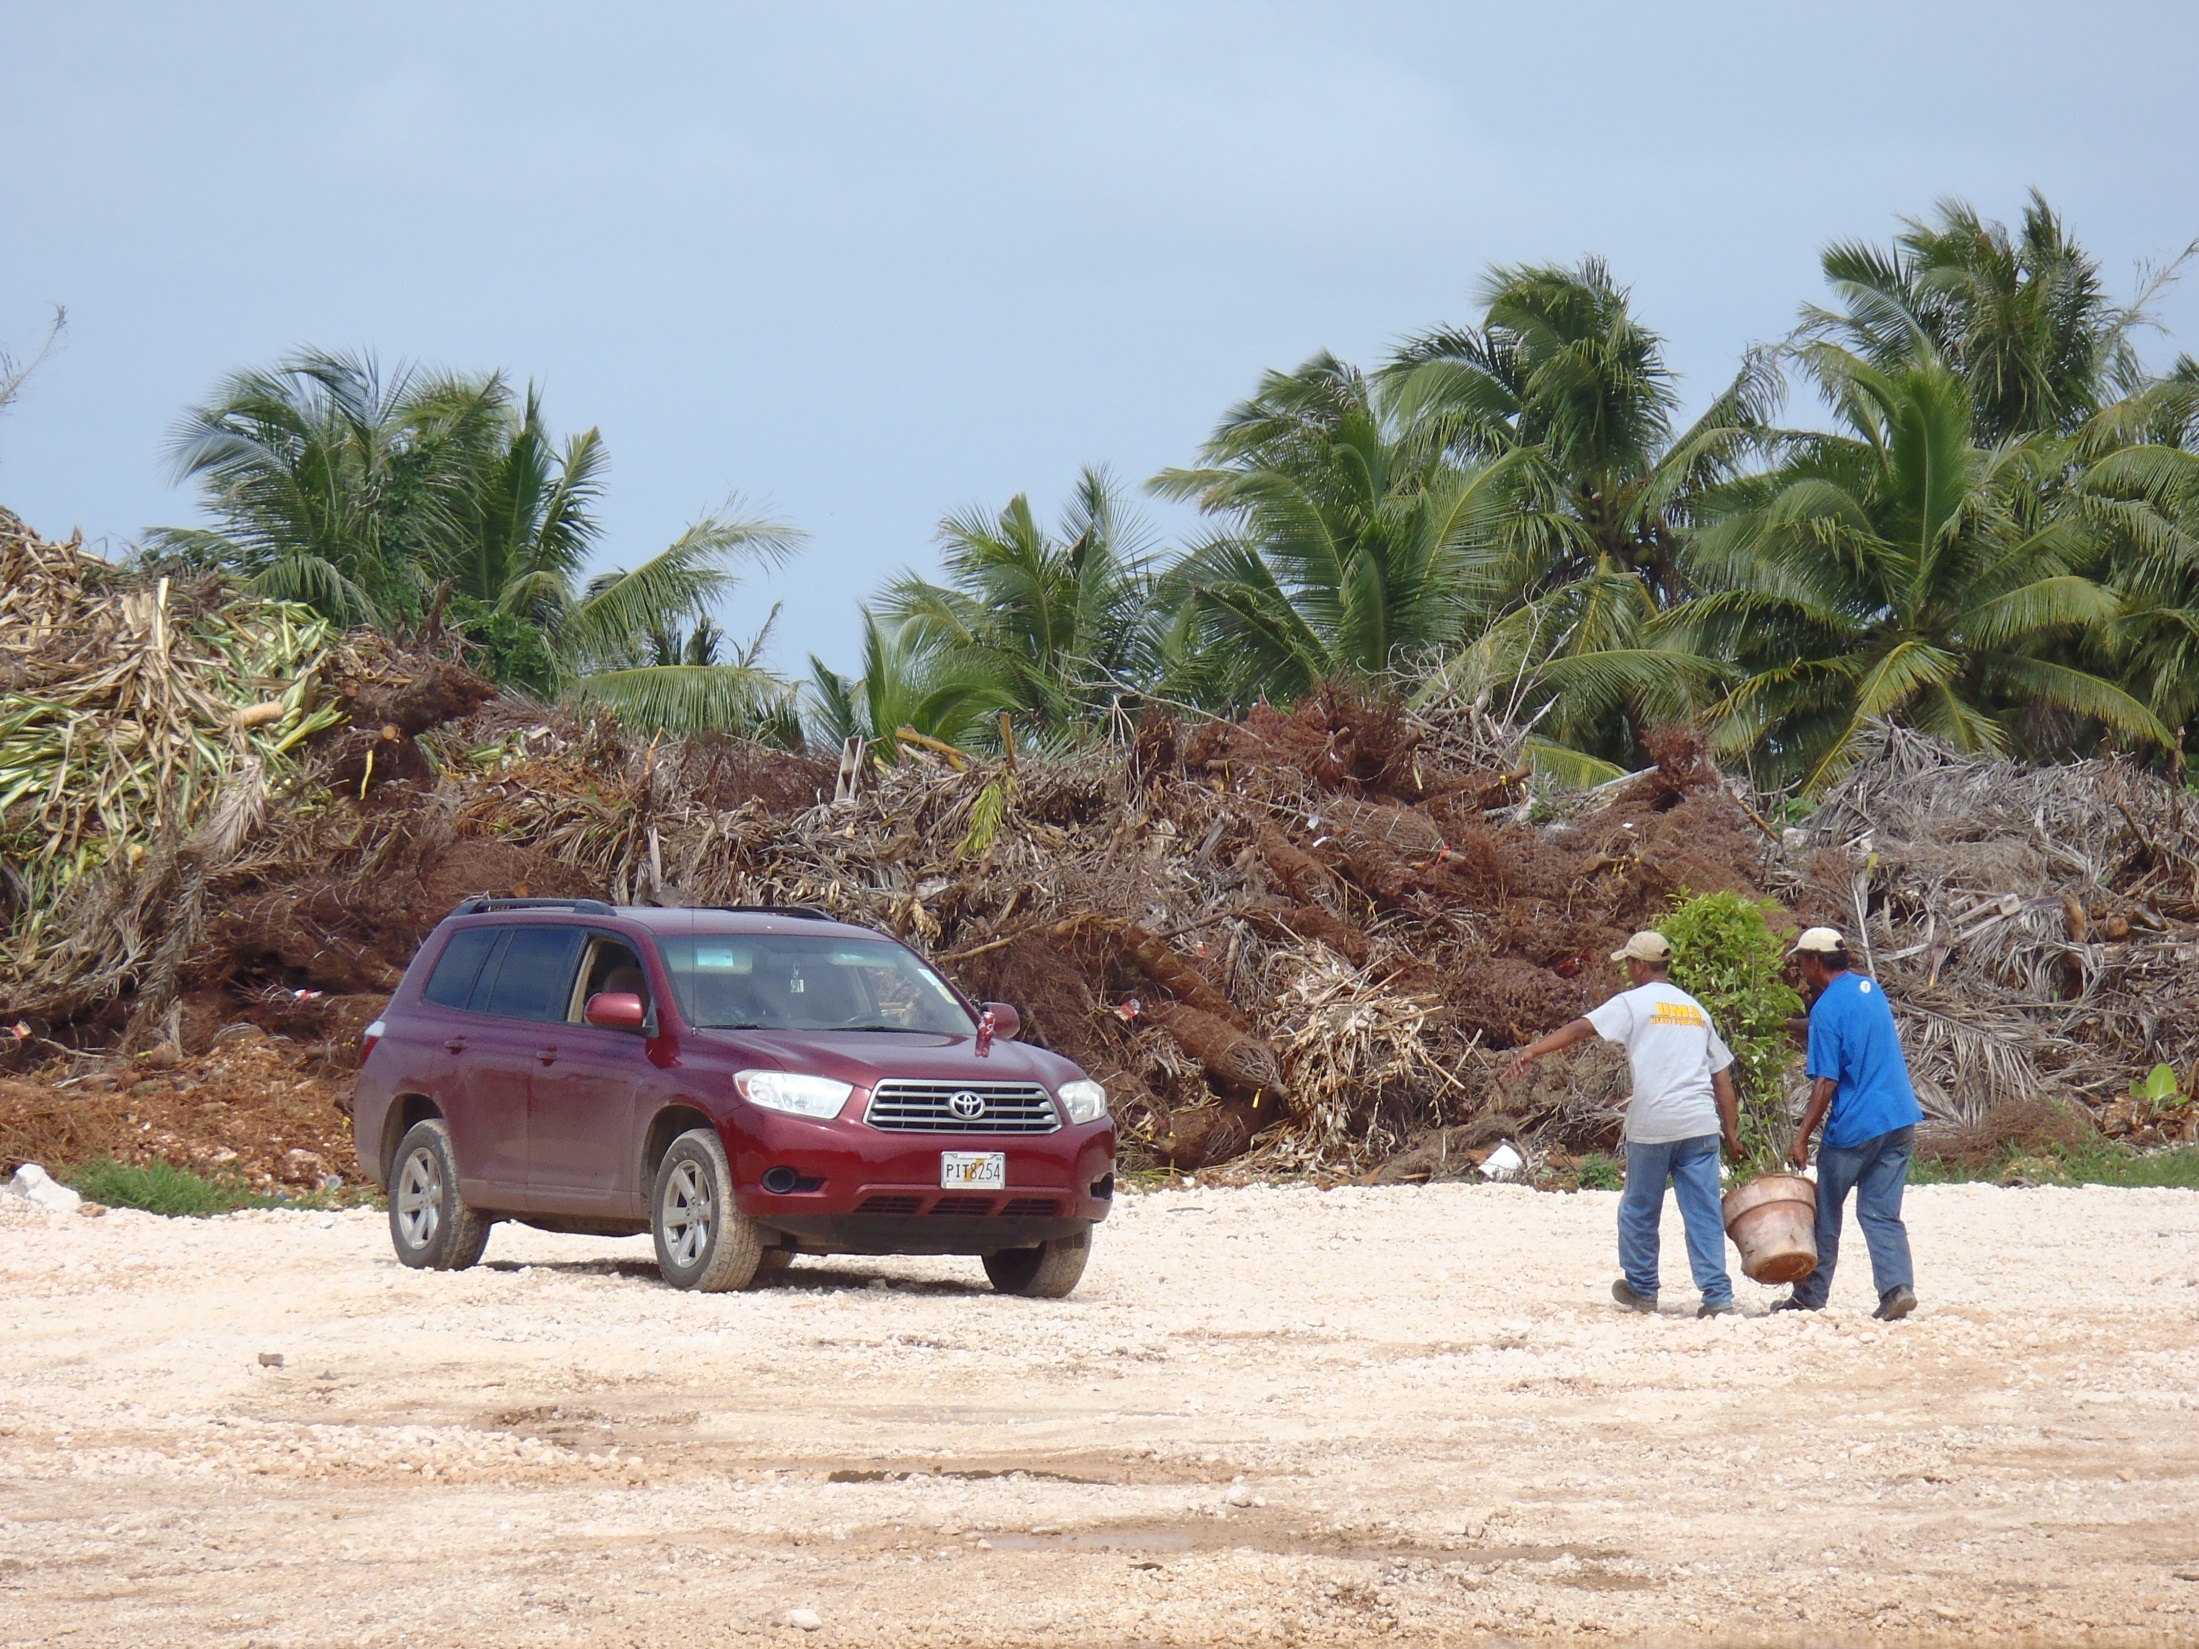
\includegraphics[height=.75\textheight]{lfa-dump.png}
%		\caption{LFA discovered by CRB crew at Primo Greenwaste Dump Site in Yigo in 2011.}
%	\end{figure}
%\end{frame}
%
%\begin{frame}{LFA - Current Status on Guam}
%	\begin{itemize}
%		\item Eradication from Guam is not feasable
%		\item LFA occurs at 20+ dispersed sites on Guam and continues to spread
%		\item Effective ant baits and application methods are available for local control programs
%	\end{itemize}
%\end{frame}
%
%\begin{frame}{LFA - Prognosis for Guam}
%	\begin{itemize}
%		\item There are no known biocontrol agents for island-wide control of LFA
%		\item Will impact quality of life for humans and pets
%		\item Possible impacts on tourism
%		\item Impacts on natural ecosystems are unpredicable
%	\end{itemize}
%\end{frame}

\section{Conclusion}

\begin{frame}{Conclusion}
	\begin{itemize}
	\item Development of IPM for invasive species which become wide-spread forest pests is difficult.
	\item Classical biocontrol may be the only feasible, stand-alone tactic.
	\end{itemize}
\end{frame}

\begin{frame}{}
\adjincludegraphics[width=\textwidth]{asian-cycad-scale/output-53.png}
\end{frame}

\end{document}
